\documentclass[a4paper,fleqn]{cas-sc}

\usepackage[authoryear,longnamesfirst]{natbib}
\usepackage{amsmath,amssymb,amsfonts,amsthm,mathtools}
\usepackage{booktabs,array,multirow}
\usepackage{graphicx}
\usepackage{microtype}
\usepackage{url}

\newtheorem{theorem}{Theorem}
\newtheorem{lemma}[theorem]{Lemma}
\newtheorem{proposition}[theorem]{Proposition}
\newtheorem{corollary}[theorem]{Corollary}
\newtheorem{assumption}{Assumption}
\newtheorem{remark}{Remark}
\DeclareMathOperator*{\argmax}{arg\,max}
\DeclareMathOperator*{\argmin}{arg\,min}
\DeclareMathOperator{\diag}{diag}
\DeclareMathOperator{\Var}{Var}
\DeclareMathOperator{\KL}{KL}
\newcommand{\E}{\mathbb E}
\newcommand{\ind}{\mathbf 1}
\newcommand{\R}{\mathbb R}
\newcommand{\T}{\mathsf T}
\newcommand{\dd}{\mathrm d}
\newcommand{\model}{\mathfrak m}
\newcommand{\D}{\mathcal D}
\newcommand{\A}{\mathcal A}
\newcommand{\PEN}{\mathcal P}
\setlength{\emergencystretch}{3em}

\begin{document}
\let\WriteBookmarks\relax
\def\floatpagepagefraction{1}
\def\textpagefraction{.001}

\shorttitle{Mixtures with component-specific response families}
\shortauthors{Pal et al.}

\title[mode=title]{Finite mixtures of generalized regressions with component-specific response families}

\author[1]{Samyajoy Pal}
\cormark[1]
\ead{palsamyajoy@gmail.com}
\author[2]{Dayasri Ravi}
\author[1]{Rouven E. Haschka}

\affiliation[1]{organization={Chair of Data Analytics, Technical University of Kaiserslautern-Landau},
  city={Kaiserslautern},
  country={Germany}}
\affiliation[2]{organization={Department of Mathematics, University of Augsburg},
  city={Augsburg},
  country={Germany}}
\cortext[1]{Corresponding author}

\begin{abstract}
Finite mixtures of generalized regressions commonly vary regression coefficients across latent components while imposing one response family on every component. That restriction can confound heterogeneity in covariate effects with heterogeneity in dispersion, tail weight, skewness, or zero inflation. We develop a frequentist framework in which each component has its own response family, link, nuisance parameters, and sparse regression vector. A penalized generalized expectation-maximization algorithm fits each candidate family tuple; response-cluster generalized linear model fits provide informed initial values, and unpenalized active-set refits supply likelihoods for Bayesian information criterion ranking. For a fixed regular tuple, we establish component and mixture identifiability under explicit separability conditions, consistency and asymptotic normality of maximum likelihood estimation, generalized expectation-maximization monotonicity, and the local non-Gaussian limit induced by lasso penalization. Louis' identity yields observed information from analytical score and Hessian blocks, which we derive for fourteen response families. Simulations show that equivalent family-tuple recovery rises toward one with sample size, lasso regularization markedly reduces false selections, and nominal 95\% Louis intervals attain coverage between 0.933 and 0.952 in three representative non-identical mixtures. In applications, a Gaussian--Gaussian--Student-$t$ model and a Poisson--negative-binomial model lead the full-data Bayesian information criterion rankings for Parkinson's telemonitoring and RAND health-utilization outcomes, respectively. Five repeated splits show stronger and more stable structural evidence for the count application than for the continuous application; complete-pipeline bootstraps quantify the remaining support and parameter uncertainty. The analysis separates fixed-model likelihood inference from the nonregular uncertainty created by family, component-number, and variable selection.
\end{abstract}

\begin{highlights}
\item Components may use different response families, links, nuisance parameters, and covariate supports.
\item Fixed-model likelihood theory is separated explicitly from nonregular family and support search.
\item Analytical Louis information is available and numerically validated for fourteen response families.
\item Simulations and two applications assess family recovery, prediction, sparsity, and bootstrap stability.
\end{highlights}

\begin{keywords}
finite mixture regression \sep heterogeneous response families \sep penalized expectation-maximization \sep variable selection \sep Louis information \sep model selection
\end{keywords}

\maketitle

\section{Introduction}
\label{sec:introduction}

Finite mixture models represent unobserved population heterogeneity by averaging a finite collection of component distributions \citep{mclachlan2000finite,mclachlan2019review}. Mixtures of regressions extend this construction by allowing latent groups to have different regression relationships. Generalized linear models (GLMs), meanwhile, connect a conditional response distribution to covariates through a link function \citep{nelder1972glm,mccullagh1989glm}. Their combination supports latent-class analysis for continuous, binary, count, and positive responses \citep{wedel1995mixture,leisch2004flexmix,grun2007fitting}. We use the term \emph{generalized regression} because our library includes classical GLM families and link-based regressions such as Student-$t$, lognormal, and skew-normal models that lie outside the strict exponential-family definition.

Most mixture regressions distinguish components through intercepts, slopes, or dispersion parameters but keep the response family common. This convention is convenient, yet it answers two scientific questions with one device: how many latent subpopulations are present, and what distributional shape is needed within each subpopulation. A homogeneous Poisson mixture, for example, may add components to absorb residual overdispersion that a negative-binomial component would represent directly. A homogeneous Gaussian mixture may similarly use extra components to approximate a heavy-tailed or skew group. Allowing component families to differ can produce a more direct account of such structure, provided that support compatibility, identifiability, optimization, and inference are treated carefully.

The idea of combining flexible component distributions is not itself new. Modular finite-mixture software permits specialized component models \citep{leisch2004flexmix,grun2007fitting}; generalized smooth mixtures allow broad parametric component families in a Bayesian construction \citep{villani2012generalized}; and recent mixture-of-experts distributional regression supports many response distributions together with covariate-dependent gating \citep{gormley2019experts,rugamer2024mixture}. Mixture-linked regressions model a response distribution through a mixture constrained by a regression mean \citep{raim2018extension}, while semiparametric mixtures relax component distributions in another direction \citep{millard2022semiparametric}. Penalized mixture regressions address component-specific variable selection \citep{khalili2007variable,stadler2010l1}, and robust, skew, overdispersed, and zero-inflated models address particular departures from a common baseline \citep{azzalini1985skew,lambert1992zip}.

The methodological gap addressed here is therefore narrower, but consequential: a unified \emph{frequentist} workflow for searching unordered tuples of non-identical response families while estimating component-specific sparse regressions, ranking active-set likelihood refits, and calculating observed information through one analytical interface. The framework must also state exactly where ordinary likelihood theory applies. In finite mixtures, coinciding components, vanishing weights, overfitted component numbers, and nested-family boundaries are singular. Variable selection adds another nonregular layer. Treating a Hessian from the selected fit as though none of these searches occurred would give a computational quantity an unjustified inferential meaning.

This paper contributes the following elements. First, it formulates a support-compatible mixture of generalized regressions in which family, link, nuisance parameters, and active predictors may differ by component. Second, it combines penalized generalized expectation-maximization (GEM), response-cluster GLM initialization, exhaustive or beam family search, and unpenalized active-set refitting. Third, it gives fixed-candidate theory under explicit assumptions: component and mixture identifiability, consistency, regular asymptotic normality, the lasso local limit, GEM monotonicity, and the scope of ordinary Bayesian information criterion (BIC) arguments. Fourth, it specializes Louis' missing-information identity to this architecture and supplies analytical derivative blocks and weighted maximization formulas for fourteen families. Fifth, it evaluates structural recovery, sparse support, predictive performance, standard errors, and coverage, and applies the same validation and bootstrap protocol to one continuous and one count dataset.

The distinction between model recovery and prediction is central throughout. BIC estimates a penalized in-sample evidence criterion; root mean squared error (RMSE) evaluates a conditional mean; and held-out log score evaluates a predictive distribution. There is no theorem requiring these rankings to agree. We report each object separately and interpret disagreement as information rather than as an implementation failure.

The remainder of the paper is organized as follows. Section~\ref{sec:methods} defines the model, computation, search, prediction, and uncertainty procedures. Section~\ref{sec:theory} gives the fixed-model theory and its limitations. Section~\ref{sec:results} presents simulations and two applications. Section~\ref{sec:discussion} concludes. Appendix~\ref{app:analytic} records the family-specific analytical Louis blocks and weighted M-step equations; complete proofs, derivations, and experiment specifications are in the standalone Supplementary Material.

\section{Methodology}
\label{sec:methods}

The methodology has three layers with different mathematical status. A fixed family tuple defines a likelihood model. Penalized GEM fits that candidate and selects component-specific supports. A discrete search then compares component numbers, family tuples, tuning parameters, and initial values. Keeping these layers distinct prevents fixed-model theory from being extended silently across a nonregular selection step.

\subsection{Fixed family-tuple model}
\label{sec:model}

Let $(Y_i,X_i)$, $i=1,\ldots,n$, be independent observations, where $Y_i\in\mathcal Y$ and $X_i\in\R^p$ includes an intercept. For a fixed component number $K$ and ordered family tuple
\[
  \model=(d_1,\ldots,d_K),
\]
all component laws are required to admit densities or masses with respect to one common sigma-finite measure $\nu$ on $\mathcal Y$. Thus continuous and count families are not mixed in the same candidate. For family $d$, write
\[
  f_d(y;\mu,\gamma),\qquad \mu=h_d(\eta)=g_d^{-1}(\eta),
\]
where $g_d$ is the link, $\mu$ is a mean or location parameter, and $\gamma$ contains family-specific nuisance parameters. Component $k$ has conditional density
\[
  q_k(y\mid x;\beta_k,\gamma_k)
  =f_{d_k}\{y;h_{d_k}(x^\T\beta_k),\gamma_k\}.
\]
The mixture regression is
\begin{equation}
  p_\theta(y\mid x)=\sum_{k=1}^K\pi_k q_k(y\mid x;\beta_k,\gamma_k),
  \qquad \pi_k>0,\quad \sum_{k=1}^K\pi_k=1,
  \label{eq:model}
\end{equation}
with parameter $\theta=\{(\pi_k,\beta_k,\gamma_k):k=1,\ldots,K\}$. The family labels $d_k$ are discrete parts of $\model$, not coordinates of $\theta$. Mixing weights are constant in the present paper; covariate-dependent gating is a distinct mixture-of-experts extension.

Table~\ref{tab:family-library} gives the implemented library. Positive nuisance parameters are optimized on a logarithmic scale and probabilities on a logit scale. For Student-$t$ components we enforce $\nu>2$, which gives finite variance and a well-defined conditional mean. The negative-binomial model uses the NB2 parameterization $\Var(Y\mid X,Z=k)=\mu+\alpha\mu^2$. ZIP and ZINB denote zero-inflated Poisson and zero-inflated negative binomial, respectively.

\begin{table}[t]
\centering
\caption{Implemented component families. The displayed link applies to the systematic parameter $\mu$; nuisance parameters are shown on their natural scale. SN, NB2, ZIP, and ZINB denote skew normal, negative binomial with quadratic variance, zero-inflated Poisson, and zero-inflated negative binomial.}
\label{tab:family-library}
\small
\begin{tabular}{llll}
\toprule
Support & Family & Link $g(\mu)$ & Nuisance parameter(s) \\
\midrule
$\R$ & Gaussian & identity & variance $\sigma^2$ \\
$\R$ & Student-$t$ & identity & scale $\sigma$, degrees $\nu>2$ \\
$\R$ & SN & identity & scale $\omega$, shape $\alpha$ \\
$(0,\infty)$ & Gamma & log & shape $\kappa$ \\
$(0,\infty)$ & exponential & log & none \\
$(0,\infty)$ & lognormal & identity on log-location & log-scale $\sigma$ \\
$(0,\infty)$ & inverse Gaussian & log & shape $\lambda$ \\
$(0,1)$ & beta & logit & precision $\phi$ \\
$\{0,1\}$ & Bernoulli & logit & none \\
$\{0,1,\ldots\}$ & Poisson & log & none \\
$\{0,1,\ldots\}$ & NB2 & log & dispersion $\alpha$ \\
$\{0,1,\ldots\}$ & geometric & log & none \\
$\{0,1,\ldots\}$ & ZIP & log & inflation $\vartheta$ \\
$\{0,1,\ldots\}$ & ZINB & log & dispersion $\alpha$, inflation $\vartheta$ \\
\bottomrule
\end{tabular}
\end{table}

Because finite mixtures are invariant to relabeling, global parameters are identifiable at most up to permutations that preserve the multiset of component families. Numerical summaries use a deterministic alignment rule; local asymptotic arguments work in a labeled neighborhood of the truth. No substantive conclusion is attached to an arbitrary component index.

\subsection{Penalized likelihood and latent-variable representation}
\label{sec:penlik}

For fixed $\model$, the observed log-likelihood is
\[
  \ell_n(\theta)=\sum_{i=1}^n\log p_\theta(Y_i\mid X_i).
\]
Let $\beta_{k,-0}$ denote all non-intercept coefficients. We maximize
\begin{equation}
  F_n(\theta)=\ell_n(\theta)-\sum_{k=1}^K\lambda_{n,k}\rho_{\alpha_k}(\beta_{k,-0}),
  \label{eq:penlik}
\end{equation}
where
\[
  \rho_\alpha(b)=\alpha\lVert b\rVert_1+\frac{1-\alpha}{2}\lVert b\rVert_2^2,
  \qquad 0\leq\alpha\leq1.
\]
The choices $\alpha=1$ and $\alpha=0$ give lasso and ridge penalties; intermediate values give elastic net. Intercepts and nuisance parameters are not penalized. Unless stated otherwise, a common $\lambda$ is used across components, while the formulation permits component-specific values. The two applications use a single lasso path, with $\alpha_k=1$ for every component when $\lambda>0$ and an unpenalized endpoint at $\lambda=0$; ridge and elastic net are not searched in the applications. Scenario B separately compares lasso and elastic net.

Introduce latent labels $Z_i\in\{1,\ldots,K\}$. Conditional on the current iterate $\theta^{(t)}$, the E-step computes
\begin{equation}
  \tau_{ik}^{(t)}=
  \frac{\pi_k^{(t)}q_k(Y_i\mid X_i;\beta_k^{(t)},\gamma_k^{(t)})}
       {\sum_{\ell=1}^K\pi_\ell^{(t)}q_\ell(Y_i\mid X_i;\beta_\ell^{(t)},\gamma_\ell^{(t)})}.
  \label{eq:responsibility}
\end{equation}
The penalized auxiliary function is
\begin{equation}
  Q_{P,n}(\theta\mid\theta^{(t)})=
  \sum_{i=1}^n\sum_{k=1}^K\tau_{ik}^{(t)}
  \{\log\pi_k+\log q_k(Y_i\mid X_i;\beta_k,\gamma_k)\}
  -\sum_{k=1}^K\lambda_{n,k}\rho_{\alpha_k}(\beta_{k,-0}).
  \label{eq:qfun}
\end{equation}
The mixing update is $\pi_k^{(t+1)}=n^{-1}\sum_i\tau_{ik}^{(t)}$. The remaining maximization separates by component into weighted generalized regressions. Closed-form, Newton, iteratively reweighted least-squares (IRLS), coordinate-descent, or low-dimensional quasi-Newton updates are used according to the family. Every accepted block update must increase $Q_{P,n}$; consequently, an inexact block gives a GEM algorithm rather than an exact expectation-maximization (EM) algorithm. Appendix~\ref{app:mstep} gives the analytical update equations.

\subsection{Initialization and convergence safeguards}
\label{sec:init}

Mixture likelihoods are multimodal, so initialization is part of the estimator's computational definition. We use two response-guided starts. The \emph{quantile--GLM} start partitions the ordered response at empirical quantiles; the \emph{$K$-means--GLM} start clusters the univariate response by $K$-means. For each resulting group and each proposed component family, a one-component weighted GLM is fitted to obtain $\beta_k$ and $\gamma_k$; group proportions initialize $\pi_k$. These values initialize the full mixture, after which responsibilities are unconstrained. Randomly perturbed starts are added in the intensive inference simulations and final refits.

Likelihood calculations use log-sum-exp evaluation. Mixing weights, scales, dispersions, shape parameters, and inflation probabilities are kept inside prespecified numerical bounds. Components with negligible weights, nonfinite predictions, nonmonotone objective steps, or failed active-set refits are flagged. A fit is declared converged only when the relative objective change meets tolerance and all validity checks pass. Because these safeguards restrict the numerical parameter space, estimates on a safeguard boundary are reported as nonregular even if the optimizer declares convergence.

\subsection{Family, component, and support search}
\label{sec:search}

Let $\D$ be a finite support-compatible family library. For small libraries we enumerate family multisets with replacement for $K=1,\ldots,K_{\max}$. Ordered assignments of a multiset to response-guided initial components may be fitted as distinct optimization starts because they can reach different local modes; structural rankings then retain the best valid fit for each multiset. For larger libraries a beam search expands the retained $(K-1)$-component tuples and carries forward the best $B$ candidates. Every candidate is fitted over the prespecified penalty grid and initialization set. Stored simulation top-ten lists retain ordered candidate fits as an optimization diagnostic, whereas application leaderboards are collapsed to unique family multisets.

Penalized fits select component-specific active sets
\[
  \widehat S_k=\{j>0:\lvert\widehat\beta_{kj}\rvert>\varepsilon\}.
\]
For each converged candidate, we then refit the unpenalized likelihood while fixing $\widehat S_1,\ldots,\widehat S_K$ and the family tuple. The Bayesian information criterion is
\begin{equation}
  \operatorname{BIC}(\model,\widehat S)
  =-2\ell_n(\widetilde\theta_{\model,\widehat S})+\widehat a_{\model}\log n,
  \qquad
  \widehat a_{\model}=(K-1)+K+\sum_{k=1}^K\lvert\widehat S_k\rvert+
  \sum_{k=1}^K\dim(\gamma_k),
  \label{eq:bic}
\end{equation}
where $K-1$ counts free mixing logits and $K$ counts component intercepts. Candidates are ranked by this active-set-refit BIC, not by the penalized objective. In the applications, a prespecified admissibility gate requires every component to retain at least one non-intercept predictor. This gate directly addresses the interpretability goal of component-specific regression and prevents a strongly penalized intercept-only component from becoming the reported scientific model. It is a design constraint, not a likelihood theorem.

Some families meet at boundaries or limits. A Student-$t$ tends to a Gaussian as its degrees of freedom diverge; NB2 tends to Poisson as $\alpha\downarrow0$; ZIP tends to Poisson as $\vartheta\downarrow0$; and ZINB tends to NB2 as $\vartheta\downarrow0$. We always report strict family-tuple matches. For selected simulation summaries we additionally report an explicitly defined equivalence match: Gaussian--Student-$t$ recognizes Student-$t$--Student-$t$, Poisson--NB2 recognizes NB2--NB2, and Poisson--ZIP recognizes ZIP--ZIP. Gamma--lognormal has no added equivalent. These equivalences are descriptive rules for family-recovery summaries, not claims that the finite-parameter probability laws are identical.

\subsection{Prediction and uncertainty}
\label{sec:inference-workflow}

Predictive log score is the held-out average of $\log p_{\widehat\theta}(y\mid x)$. RMSE and mean absolute error (MAE) use the family-correct mixture mean
\[
  \widehat m(x)=\sum_{k=1}^K\widehat\pi_k m_{d_k}(x;\widehat\beta_k,\widehat\gamma_k).
\]
For Gaussian and Student-$t$, $m_d=\mu$; for skew normal, $m_d=\mu+\omega\delta\sqrt{2/\pi}$ with $\delta=\alpha/\sqrt{1+\alpha^2}$; for lognormal, $m_d=\exp(\mu+\sigma^2/2)$; and for ZIP or ZINB, $m_d=(1-\vartheta)\mu$. The other mean-parameterized families use $m_d=\mu$. This distinction avoids scoring a location parameter as though it were a predictive mean.

Two uncertainty summaries serve different targets. In a fixed regular candidate, analytical Louis information estimates the covariance of the unpenalized maximum likelihood estimator. After model search and penalization, its inverse is only a conditional diagnostic. The application-level uncertainty analysis therefore uses a complete-pipeline nonparametric bootstrap: the validated family tuple is held fixed, but predictor screening, penalty choice, support selection, active-set refitting, and label alignment are repeated in each bootstrap sample. Participants, rather than recordings, are resampled for the longitudinal Parkinson data. The resulting percentile intervals incorporate support and tuning variability conditional on the selected family tuple; they do not incorporate uncertainty from repeating the family and component-number search.

\section{Theoretical properties}
\label{sec:theory}

The results in this section concern one fixed family tuple $\model=(d_1,\ldots,d_K)$ and one fixed finite-dimensional coefficient support. This is the regime in which ordinary likelihood arguments can be made precise. Family search, component-number search, boundary approximations, and data-dependent support selection are excluded from the theorem statements and addressed separately in the remarks and bootstrap design.

\subsection{Assumptions and identifiability}
\label{sec:assumptions}

Identifiability of a heterogeneous mixture cannot be obtained from full-rank regressors alone. It requires both identifiability of each primitive regression and separability of finite mixtures formed from the proposed component classes. We state both requirements explicitly.

\begin{assumption}[Regular fixed candidate]
\label{ass:regular}
For the fixed tuple $\model$ and a labeled parameter space $\Theta_{\model}$, the following conditions hold.
\begin{enumerate}
\item[(A1)] The pairs $(Y_i,X_i)$ are independent and identically distributed, and $Y_i\mid X_i=x$ has density $p_{\theta_0}(\cdot\mid x)$ for some $\theta_0\in\Theta_{\model}$.
\item[(A2)] The labeled space $\Theta_{\model}$ is compact, $\theta_0$ is an interior point, and $\pi_k\geq\pi_{\min}>0$. Scales and dispersions are bounded away from zero and infinity, inflation probabilities are bounded away from zero and one, and distinct true component atoms do not coincide.
\item[(A3)] For every $(y,x)$ in the common support, $p_\theta(y\mid x)>0$ and $\log p_\theta(y\mid x)$ is continuous in $\theta$. The class $\{\log p_\theta:\theta\in\Theta_{\model}\}$ is Glivenko--Cantelli under the true joint law; equivalently, the uniform law of large numbers used below holds.
\item[(A4)] Each primitive family is identifiable in $(\mu,\gamma)$; its inverse link $h_d$ is one-to-one; and $X^\T b=0$ almost surely implies $b=0$.
\item[(A5)] The union of component regression classes in $\model$ is $K$-identifiable: equality almost everywhere of two mixtures containing at most $K$ positive, distinct atoms implies equality of their weighted density functions up to a permutation. It is also cross-family separable in the parameter interior: equal primitive regression densities from two proposed classes must have the same family label and, by (A4), the same regression and nuisance parameters.
\end{enumerate}
\end{assumption}

Condition (A5) is a substantive model condition rather than a generic property of every arbitrary collection of distributions. It is related to linear independence of component densities and to classical finite-mixture identifiability \citep{teicher1963identifiability,hennig2000identifiability}. It must be verified or assumed for the particular tuple under study. It can fail when components coincide or when one proposed representation lies on a nested-family boundary, which is why those cases are excluded from the regular theory.

\begin{lemma}[Primitive regression identifiability]
\label{lem:primitive}
Under (A4), equality
\[
 f_d\{y;h_d(x^\T\beta_1),\gamma_1\}
 =f_d\{y;h_d(x^\T\beta_2),\gamma_2\}
\]
for $P_X$-almost every $x$ and $\nu$-almost every $y$ implies $(\beta_1,\gamma_1)=(\beta_2,\gamma_2)$.
\end{lemma}

\begin{theorem}[Identifiability of a fixed family tuple]
\label{thm:ident}
Under (A4) and (A5), the restriction of the fixed-tuple model to representations with $K$ positive, distinct component atoms is identifiable up to a permutation of component labels. Moreover, a distribution represented by $K$ positive, distinct atoms cannot have an equivalent representation with fewer than $K$ distinct atoms from the proposed classes.
\end{theorem}

Assumption (A5) first matches the weighted component densities and rules out cross-family aliases; Lemma~\ref{lem:primitive} then identifies each nuisance parameter and linear predictor, after which the random-design condition identifies its coefficient vector. The distinct-atom restriction is essential: splitting one atom into duplicate copies makes the unrestricted parameterization nonidentifiable. Supplementary Section~S1 gives the complete argument and shows why a redundant representation cannot equal a $K$-distinct-atom truth.

\subsection{Consistency and regular asymptotic normality}
\label{sec:regular-theory}

The population conditional log-likelihood differs from its value at the truth by a conditional Kullback--Leibler divergence. Compactness, the uniform law of large numbers, and the preceding identifiability result therefore produce a standard but fully delimited M-estimation problem.

\begin{theorem}[Existence and consistency]
\label{thm:consistency}
Under (A1)--(A5), an unpenalized maximizer $\widehat\theta_n\in\argmax_{\theta\in\Theta_{\model}}\ell_n(\theta)$ exists whenever the sample criterion is finite. Under the labeling convention,
\[
  \widehat\theta_n\xrightarrow{p}\theta_0.
\]
\end{theorem}

For a distributional limit, the local model must be separated from every mixture singularity. The following differentiability assumption is intentionally stronger than the consistency conditions.

\begin{assumption}[Local likelihood regularity]
\label{ass:local}
In a labeled neighborhood of $\theta_0$, the free parameter is an open subset of $\R^r$. The log density is twice continuously differentiable, its first two derivatives admit integrable local envelopes, the score has finite second moment, and
\[
 I(\theta_0)=\E_{\theta_0}\{S_{\theta_0}(Y,X)S_{\theta_0}(Y,X)^\T\},
 \qquad S_\theta=\nabla_\theta\log p_\theta(Y\mid X),
\]
is nonsingular. The local maximum likelihood estimator solves the score equation with probability tending to one.
\end{assumption}

\begin{theorem}[Asymptotic normality in the regular fixed model]
\label{thm:normal}
Under Assumptions~\ref{ass:regular} and \ref{ass:local},
\[
  \sqrt n(\widehat\theta_n-\theta_0)
  \rightsquigarrow N\{0,I(\theta_0)^{-1}\}.
\]
\end{theorem}

The proof expands the score at $\theta_0$, applies the multivariate central limit theorem to the score, and proves convergence of the intermediate Hessian by consistency and the derivative envelopes. The complete proof is given in Supplementary Section~S1. The theorem excludes zero weights, coincident components, singular information, and nuisance estimates on imposed bounds.

\subsection{Analytical observed information}
\label{sec:louis}

Directly differentiating a log of heterogeneous component sums is possible but numerically fragile. Louis' identity rewrites the observed information as complete-data curvature minus the information lost through the unobserved labels \citep{louis1982information}. The same identity applies to every family once its component score and Hessian are supplied.

For observation $i$, define
\[
 c_{ik}(\theta)=\log\pi_k+\log q_k(Y_i\mid X_i;\beta_k,\gamma_k),
 \quad s_{ik}=\nabla_\theta c_{ik},
 \quad H_{ik}=\nabla_\theta^2c_{ik},
\]
and let $\tau_{ik}$ be given by \eqref{eq:responsibility} at $\theta$. Entries outside component $k$ are zero except for the shared mixing-logit coordinates.

\begin{theorem}[Louis identity for a finite regression mixture]
\label{thm:louis}
Under the fixed-model differentiability conditions, the observed information contribution of observation $i$ is
\begin{equation}
 I_i(\theta)=
 -\sum_{k=1}^K\tau_{ik}H_{ik}
 -\sum_{k=1}^K\tau_{ik}(s_{ik}-\bar s_i)(s_{ik}-\bar s_i)^\T,
 \qquad
 \bar s_i=\sum_{k=1}^K\tau_{ik}s_{ik}.
 \label{eq:louis}
\end{equation}
Consequently $I_{\mathrm{obs},n}(\theta)=\sum_i I_i(\theta)$ equals
\[
 -\E_\theta\{\nabla_\theta^2\ell_{c,n}(\theta)\mid Y,X\}
 -\Var_\theta\{\nabla_\theta\ell_{c,n}(\theta)\mid Y,X\}.
\]
\end{theorem}

The negative second term in \eqref{eq:louis} is the missing-information correction. It is essential: using only the responsibility-weighted component Hessians overstates information because it treats posterior labels as observed.

The family interface is defined in scalar systematic coordinates. For $\ell=\log f(y;\mu,\gamma)$, let
\[
 a_\mu=\partial_\mu\ell,\quad b_{\mu\mu}=\partial_{\mu\mu}^2\ell,
 \quad a_\gamma=\nabla_\gamma\ell,\quad
 B_{\gamma\gamma}=\nabla_{\gamma\gamma}^2\ell,
 \quad b_{\mu\gamma}=\nabla_\gamma(\partial_\mu\ell).
\]

\begin{proposition}[Regression-coordinate chain rule]
\label{prop:chain}
Let $\eta=x^\T\beta$, $\mu=h(\eta)$, and write $\dot h$ and $\ddot h$ for derivatives of the inverse link. Then
\[
 s_\beta=x\,a_\mu\dot h,\qquad s_\gamma=a_\gamma,
\]
\[
 H_{\beta\beta}=xx^\T\{b_{\mu\mu}\dot h^2+a_\mu\ddot h\},\qquad
 H_{\beta\gamma}=x\{\dot h\,b_{\mu\gamma}\}^\T,
 \qquad H_{\gamma\gamma}=B_{\gamma\gamma}.
\]
\end{proposition}

For $K-1$ free mixing logits $a_j$, with $a_K=0$,
\[
 \frac{\partial\log\pi_k}{\partial a_j}=\ind\{k=j\}-\pi_j,
 \qquad
 \frac{\partial^2\log\pi_k}{\partial a\,\partial a^\T}
 =-\{\diag(\pi_{1:K-1})-\pi_{1:K-1}\pi_{1:K-1}^\T\}.
\]
Theorem~\ref{thm:louis}, Proposition~\ref{prop:chain}, and the family blocks in Appendix~\ref{app:analytic} therefore give a fully analytical observed-information matrix. In a regular unpenalized model, $I_{\mathrm{obs},n}(\widehat\theta_n)^{-1}$ estimates $\Var(\widehat\theta_n)$. After search or penalization it is reported only as a conditional diagnostic.

\subsection{Penalization changes the limiting law}
\label{sec:penalty-theory}

An $\ell_1$ penalty is nondifferentiable at zero. Even in a regular fixed mixture, the raw penalized estimator is not generally asymptotically Gaussian at truly zero coordinates \citep{knight2000asymptotics,leeb2005selection}. The relevant scaling depends on whether the objective uses the sum log-likelihood, as in \eqref{eq:penlik}.

\begin{proposition}[Local limit under lasso penalization]
\label{prop:lasso}
Suppose the regular fixed-model assumptions hold, and let $\widehat\theta_{n,\lambda}$ be a consistent local maximizer. Let $\PEN$ be the penalized coordinates and permit coordinate-specific tuning constants satisfying $\lambda_{n,j}/\sqrt n\to\lambda_j\in[0,\infty)$. Then $\sqrt n(\widehat\theta_{n,\lambda}-\theta_0)$ converges to the almost surely unique maximizer of
\begin{equation}
 u^\T Z-\frac12u^\T I(\theta_0)u-
 \sum_{j\in\PEN}\lambda_j
 \left[u_j\operatorname{sign}(\theta_{0j})\ind\{\theta_{0j}\neq0\}
 +|u_j|\ind\{\theta_{0j}=0\}\right],
 \label{eq:lasso-limit}
\end{equation}
where $Z\sim N\{0,I(\theta_0)\}$. If every $\lambda_{n,j}/\sqrt n\to0$, the usual Gaussian limit is recovered. If some $\lambda_j>0$ at a true zero, the limit is generally non-Gaussian.
\end{proposition}

This result rules out naive Louis-Wald intervals for the raw lasso estimator under selection-scale penalization. An unpenalized refit removes the penalty kink only conditionally on the selected support; it does not erase selection uncertainty. That is why the experiments assess fixed-model Wald coverage separately from the application bootstrap.

\subsection{GEM ascent and the scope of BIC}
\label{sec:algorithm-theory}

The computation supplies an ascent guarantee, not a global-mode guarantee. Likewise, ordinary BIC consistency applies only to regular candidates and does not resolve singular mixture order or nested-family boundaries.

\begin{theorem}[Penalized GEM monotonicity]
\label{thm:gem}
If an update satisfies
\[
 Q_{P,n}(\theta^{(t+1)}\mid\theta^{(t)})
 \geq Q_{P,n}(\theta^{(t)}\mid\theta^{(t)}),
\]
then $F_n(\theta^{(t+1)})\geq F_n(\theta^{(t)})$. If the parameter space is compact, $F_n$ is continuous, the update map is closed, and every nonstationary point has a neighborhood on which one full update increases $F_n$ by a uniformly positive amount, every accumulation point of the GEM sequence is stationary.
\end{theorem}

The proof uses the conditional Kullback--Leibler decomposition underlying EM and a contradiction argument for a nonstationary accumulation point, following the convergence logic of \citet{dempster1977em} and \citet{wu1983convergence}. It does not assert convergence to the global maximum, hence the use of informed and repeated starts.

\begin{proposition}[BIC for a finite regular candidate collection]
\label{prop:bic}
Consider finitely many fixed, regular candidates. Suppose that the true model is included, every incorrect nonnested candidate has a positive Kullback--Leibler gap, and every larger candidate containing the truth has an ordinary $O_p(1)$ Wilks-type likelihood gain. Then BIC selects the smallest true candidate with probability tending to one.
\end{proposition}

Proposition~\ref{prop:bic} excludes the most delicate comparisons in the empirical search: extra mixture components, zero mixing weights, coincident components, and Poisson/NB2 or ordinary/zero-inflated boundaries. Classical mixture-order results require specialized conditions \citep{keribin2000order}, and singular criteria require different asymptotics \citep{drton2017sbic}. Equation~\eqref{eq:bic} is therefore a transparent practical ranking rule for the full search, not a claimed solution to post-search inference or singular model-selection theory.

\section{Results}
\label{sec:results}

The empirical study evaluates four claims separately: recovery of a non-identical family structure, component-specific variable selection, fixed-model likelihood inference, and evidence of heterogeneous response families in data. All reported summaries come from frozen, complete runs. Failed or nonfinite fits are retained in computation diagnostics but excluded under prespecified validity rules; exact denominators and settings are reported below and in the Supplementary Material.

\subsection{Simulation study}
\label{sec:simulation}

The simulation is divided into three scenarios because model selection, prediction, support recovery, and standard-error calibration have different targets. Scenario A searches the candidate family space, Scenario B fixes the family tuple and studies sparsity, and Scenario C fixes the regular data-generating tuple and studies Louis-Wald inference.

\subsubsection{Design}

Four two-component data-generating models are used: Gaussian--Student-$t$, Gamma--lognormal, Poisson--NB2, and Poisson--ZIP. Mixing weights range from 0.40 to 0.60. Non-intercept covariates are Gaussian with autoregressive correlation $0.2^{|a-b|}$. Scenario A uses $p=5$, sample sizes $n\in\{500,1000,1500\}$, 100 Monte Carlo replications, and an independent test sample of size 2000. Within each support class, it searches one to three components. The candidate sets are Gaussian/Student-$t$/skew normal for real responses, Gamma/lognormal/inverse Gaussian for positive responses, and Poisson/NB2/ZIP for counts. A beam width of 10 and two starts per candidate are used.

Scenario B uses $n=1000$, $p=20$, 100 replications, and the true family tuple. Each component has four active slopes and 15 null slopes. It compares no penalty, lasso, and elastic net, selecting within each penalty class by BIC. Scenario C uses unpenalized fits of the true tuple. Gaussian--Student-$t$ and Poisson--ZIP use 100 replications at each of $n=500,1000,1500$; an intensive Gamma--lognormal run uses 500 replications at $n=500,1000,1500,2500$, 50 starts from response-cluster GLM initializations, and up to 250 GEM iterations. This intensive run was prespecified after diagnosing local-mode contamination in a lower-start run; it replaces, rather than supplements, the contaminated Gamma--lognormal inference summary. Supplementary Section~S3 gives every coefficient, nuisance parameter, tuning value, seed, convergence rule, and equivalence definition.

\subsubsection{Family recovery and predictive ranking}

Family-tuple recovery improves with sample size, but strict and scientifically equivalent recovery differ when families meet at a boundary. Table~\ref{tab:sim-selection} reports both, together with the probability that a strict or equivalent generating tuple appears in the ten best candidates under BIC and held-out log score.

\begin{table}[t]
\centering
\caption{Scenario A family-tuple selection over 100 replications. ``Equivalent'' applies only the prespecified summary rules in Section~\ref{sec:search}. Top-ten columns give inclusion of the strict or equivalent generating tuple among the ten best ordered candidate fits.}
\label{tab:sim-selection}
\small
\begin{tabular}{llrrrr}
\toprule
Generating tuple & $n$ & Strict & Equivalent & BIC top 10 & Log-score top 10 \\
\midrule
Gaussian--Student-$t$ & 500  & .75 & .75 & 1.00 & 1.00 \\
 & 1000 & .96 & .96 & 1.00 & .99 \\
 & 1500 & .99 & .99 & 1.00 & .98 \\
Gamma--lognormal & 500  & .56 & .56 & 1.00 & .98 \\
 & 1000 & .68 & .68 & .98 & .98 \\
 & 1500 & .81 & .81 & .95 & .95 \\
Poisson--NB2 & 500  & .00 & .48 & 1.00 & 1.00 \\
 & 1000 & .00 & .88 & 1.00 & 1.00 \\
 & 1500 & .00 & .98 & 1.00 & 1.00 \\
Poisson--ZIP & 500  & 1.00 & 1.00 & 1.00 & 1.00 \\
 & 1000 & .99 & .99 & 1.00 & 1.00 \\
 & 1500 & .99 & .99 & 1.00 & 1.00 \\
\bottomrule
\end{tabular}
\end{table}

Gaussian--Student-$t$ strict recovery rises from 0.75 to 0.99; Gamma--lognormal rises more slowly from 0.56 to 0.81; and Poisson--ZIP is recovered in at least 0.99 of replications. The zero strict rate for Poisson--NB2 is not a complete failure of distributional recovery: BIC usually selects NB2--NB2, with one fitted dispersion close to the Poisson limit. Under the declared boundary-equivalence rule, recovery rises from 0.48 to 0.98. Strict results remain visible so that the equivalence convention cannot manufacture exact recovery.

Figure~\ref{fig:simulation} also shows that the BIC winner is the held-out log-score winner in only 0.18--0.72 of replications. The agreement rate does not increase uniformly with $n$. BIC rewards a parsimonious approximation to the generating distribution, while held-out log score ranks realized predictive density; neither criterion is designed to optimize the other. The stronger computational diagnostic is that the generating or equivalent tuple appears in both top-ten candidate-fit lists with probability at least 0.95 in every reported configuration.

\begin{figure}[t]
\centering
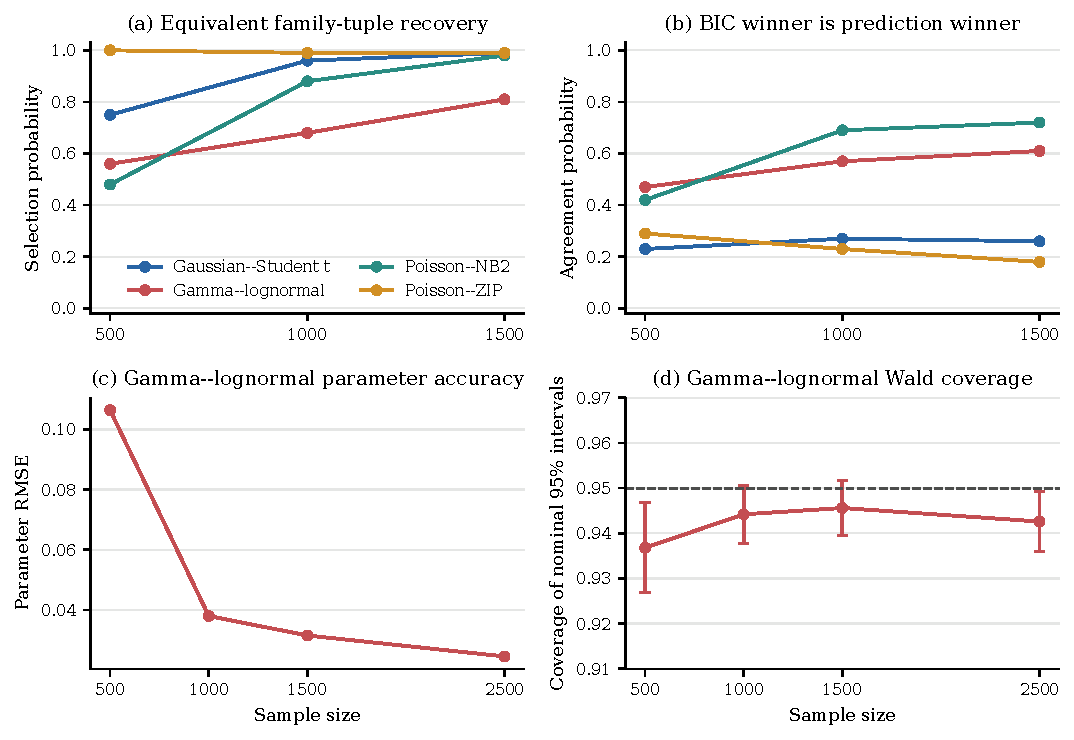
\includegraphics[width=\linewidth]{fig1.pdf}
\caption{Simulation behavior with increasing sample size. (a) Prespecified equivalence-class family recovery in Scenario A. (b) Probability that the BIC winner is also the held-out log-score winner. (c) Parameter root mean squared error (RMSE) for the intensive Gamma--lognormal inference run. (d) Empirical coverage of nominal 95\% analytical-Louis Wald intervals for that run; vertical bars are 95\% Monte Carlo intervals and the dashed line is 0.95.}
\label{fig:simulation}
\end{figure}

\subsubsection{Component-specific variable selection}

The sparse experiment shows the expected distinction between fitting a dense likelihood and recovering a support. Table~\ref{tab:sim-selection-vars} and Figure~\ref{fig:variables} summarize true-positive rate (TPR), false-positive rate (FPR), false-discovery rate (FDR), total selected slopes, and test log score.

\begin{table}[t]
\centering
\caption{Scenario B variable selection at $n=1000$ over 100 replications. Selected is the mean number of slopes retained across both components; the true total is eight. Test log score is held-out average log likelihood per observation.}
\label{tab:sim-selection-vars}
\small
\begin{tabular}{llrrrrr}
\toprule
Generating tuple & Penalty & TPR & FPR & FDR & Selected & Test log score \\
\midrule
Gaussian--Student-$t$ & None & 1.000 & .998 & .750 & 39.95 & -1.919 \\
 & Lasso & 1.000 & .222 & .388 & 16.66 & -1.915 \\
 & Elastic net & 1.000 & .524 & .602 & 25.72 & -1.917 \\
Gamma--lognormal & None & 1.000 & .995 & .749 & 39.84 & -1.152 \\
 & Lasso & .717 & .152 & .289 & 11.74 & -1.170 \\
 & Elastic net & .766 & .276 & .494 & 15.93 & -1.165 \\
Poisson--ZIP & None & 1.000 & .997 & .749 & 39.92 & -2.477 \\
 & Lasso & .975 & .297 & .452 & 18.67 & -2.473 \\
 & Elastic net & .985 & .383 & .520 & 21.33 & -2.473 \\
\bottomrule
\end{tabular}
\end{table}

\begin{figure}[t]
\centering
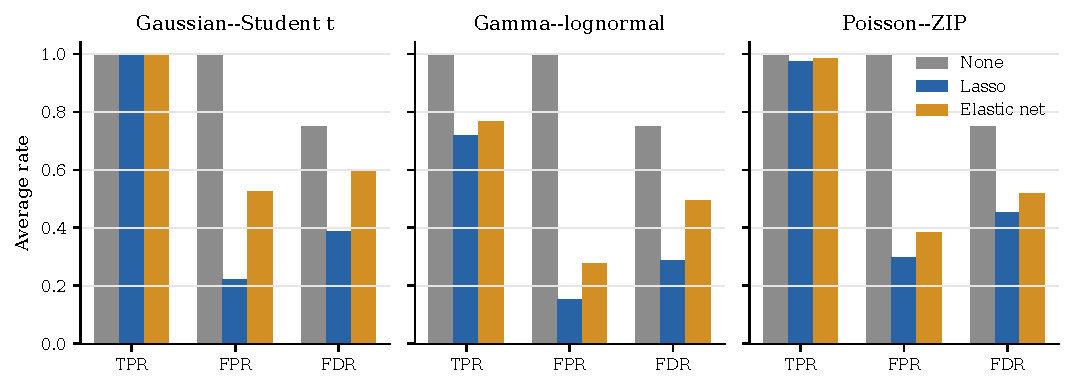
\includegraphics[width=\linewidth]{fig2.pdf}
\caption{Scenario B support recovery. TPR, FPR, and FDR denote true-positive, false-positive, and false-discovery rates. Lasso produces the lowest FPR and FDR in each design; elastic net retains somewhat more signal and more null slopes in the two harder designs.}
\label{fig:variables}
\end{figure}

Without penalization nearly every null slope is retained. Lasso reduces FPR to 0.152--0.297 while retaining all signals in Gaussian--Student-$t$, 71.7\% in Gamma--lognormal, and 97.5\% in Poisson--ZIP. Elastic net is consistently less sparse and slightly increases TPR in the latter two designs. Prediction changes little in Gaussian--Student-$t$ and Poisson--ZIP; in Gamma--lognormal, the dense fit has the better log score. Penalization is therefore effective structural regularization here, but it is not uniformly predictive.

\subsubsection{Analytical Louis inference}

Fixed-model inference is evaluated only after fixing the correct $K$, family tuple, and full coefficient support. Table~\ref{tab:sim-inference} reports analytical Louis results. For Gaussian--Student-$t$ and Poisson--ZIP, central numerical-Hessian standard errors agree with analytical values to the displayed precision in every configuration and both methods succeed in all replications. The fourteen family derivative blocks also pass direct score/Hessian finite-difference validation; the largest absolute discrepancy over the validation suite is $1.1\times10^{-5}$ (Supplementary Table~S3).

\begin{table}[t]
\centering
\caption{Scenario C analytical Louis inference for all free parameters. MAB is mean absolute bias, SE is mean standard error, and coverage is for nominal 95\% Wald intervals. Gaussian--Student-$t$ and Poisson--ZIP use 100 replications; Gamma--lognormal uses 500.}
\label{tab:sim-inference}
\small
\begin{tabular}{lrrrrr}
\toprule
Generating tuple & $n$ & MAB & Mean SE & Coverage & Mean interval length \\
\midrule
Gaussian--Student-$t$ & 500  & .0752 & .0926 & .9370 & .3630 \\
 & 1000 & .0521 & .0648 & .9480 & .2540 \\
 & 1500 & .0439 & .0544 & .9520 & .2131 \\
Gamma--lognormal & 500  & .0420 & .0437 & .9368 & .1712 \\
 & 1000 & .0247 & .0310 & .9442 & .1216 \\
 & 1500 & .0204 & .0253 & .9456 & .0993 \\
 & 2500 & .0159 & .0196 & .9426 & .0768 \\
Poisson--ZIP & 500  & .0599 & .0715 & .9430 & .2802 \\
 & 1000 & .0414 & .0489 & .9330 & .1916 \\
 & 1500 & .0316 & .0386 & .9380 & .1512 \\
\bottomrule
\end{tabular}
\end{table}

Bias, mean SE, and interval length decrease with sample size in all three designs. Coverage ranges from 0.933 to 0.952 and is not monotonically increasing, as expected within Monte Carlo variation and finite-mixture finite-sample effects. In the 500-replication Gamma--lognormal run, coverage is 0.9368--0.9456 while parameter RMSE falls from 0.1064 at $n=500$ to 0.0245 at $n=2500$. These results support the analytical information calculation in regular fixed models; they do not validate Wald inference after the family or support search.

\subsection{Applications}
\label{sec:applications}

The applications use one common reporting template. Each dataset has five 80/20 splits, a full-data exhaustive leaderboard, and one lasso path. Specifically, the penalty in \eqref{eq:penlik} has $\alpha_k=1$ for every component and a common tuning value $\lambda\in\{0,0.1,0.25,0.5,1,2,5,10,20\}$, where $\lambda=0$ is the unpenalized endpoint. No ridge or elastic-net application fits enter the reported searches. Each leaderboard candidate also uses two response-guided starts, the active-component gate, family-correct log score/RMSE/MAE, analytical Louis diagnostics, and 500 complete-pipeline bootstrap samples. Table~\ref{tab:app-full} compares the full-data selections; Table~\ref{tab:app-prediction} and Figure~\ref{fig:splits} compare split behavior. Figure~\ref{fig:leaders} displays the ten best unique family tuples by full-data BIC.

\begin{figure}[t]
\centering
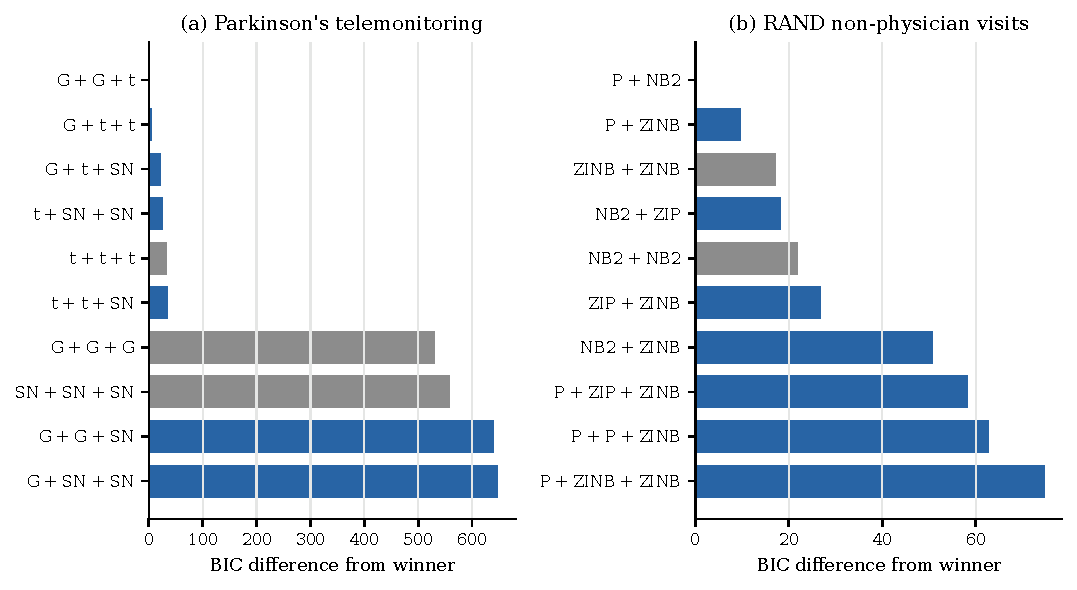
\includegraphics[width=\linewidth]{fig3.pdf}
\caption{Full-data application leaderboards. For each unique family tuple, the best admissible active-set-refit BIC is shown relative to the winner. Blue bars denote non-identical tuples and gray bars identical-family tuples. G, $t$, SN, P, NB2, ZIP, and ZINB denote Gaussian, Student-$t$, skew normal, Poisson, negative binomial with quadratic variance, zero-inflated Poisson, and zero-inflated negative binomial.}
\label{fig:leaders}
\end{figure}

\begin{table}[t]
\centering
\caption{Full-data application results under the common active-component gate. BIC differences are positive in favor of the selected non-identical tuple. Selection BIC uses the common leaderboard start budget. The RAND expanded refit adds starts only after selection and is not used to rerank competitors.}
\label{tab:app-full}
\small
\begin{tabular}{lrrrrrr}
\toprule
Dataset and selected tuple & $\lambda$ & Selection BIC & vs. identical & vs. $K=1$ & Final weights & Active slopes \\
\midrule
Parkinson: G+G+$t$ & 10 & 3088.0 & 32.1 & 2047.6 & .328/.269/.403 & 17/15/13 \\
RAND: P+NB2 & 20 & 7949.5 & 17.1 & 549.7 & .865/.135 & 24/10 \\
\bottomrule
\end{tabular}
\end{table}

\begin{figure}[t]
\centering
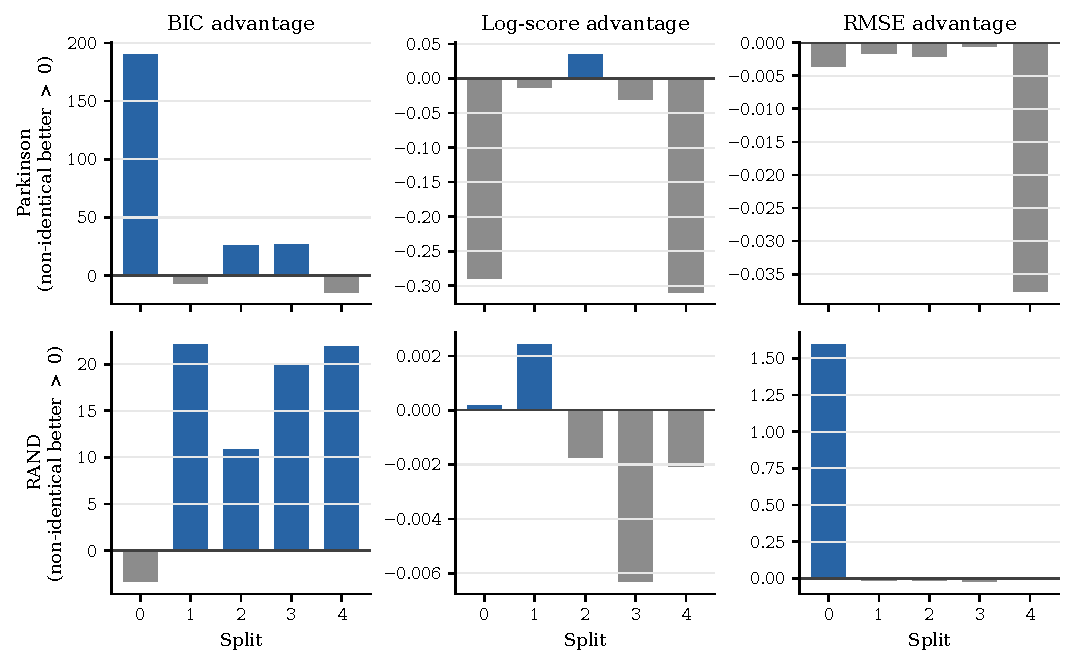
\includegraphics[width=\linewidth]{fig4.pdf}
\caption{Five-split validation. Within each split, the best admissible non-identical candidate is compared with the best admissible identical-family candidate having $K>1$. Positive values favor the non-identical model. BIC, held-out log score, and RMSE deliberately measure different targets.}
\label{fig:splits}
\end{figure}

\begin{table}[t]
\centering
\caption{Mean held-out performance of the BIC-best member of each model class across five splits. Log score is average held-out log likelihood per observation. Lower RMSE and MAE are better.}
\label{tab:app-prediction}
\small
\begin{tabular}{llrrr}
\toprule
Dataset & Model class & Log score & RMSE & MAE \\
\midrule
Parkinson & $K=1$ & -1.3060 & .5364 & .4550 \\
 & Identical, $K>1$ & -1.5765 & .5168 & .4394 \\
 & Non-identical & -1.6980 & .5259 & .4490 \\
RAND & $K=1$ & -.7652 & 3.0189 & .8708 \\
 & Identical, $K>1$ & -.6596 & 3.3146 & .8780 \\
 & Non-identical & -.6611 & 3.0070 & .8516 \\
\bottomrule
\end{tabular}
\end{table}

\subsubsection{Parkinson's telemonitoring}

The Parkinson's telemonitoring data contain 5875 voice recordings from 42 participants with early-stage Parkinson's disease \citep{uci2009parkinsons,tsanas2010parkinsons}. The response is the logarithm of total Unified Parkinson's Disease Rating Scale (UPDRS). The 17 candidate slopes comprise age, sex, time since recruitment, jitter and shimmer summaries, the noise-to-harmonics ratio (NHR), the harmonics-to-noise ratio (HNR), recurrence period density entropy (RPDE), detrended fluctuation analysis (DFA), and pitch period entropy (PPE). In the jitter and shimmer labels, RAP denotes relative average perturbation, PPQ5 the five-point period perturbation quotient, and APQ an amplitude perturbation quotient. Jitter:DDP and Shimmer:DDA are excluded because they are exact linear transformations of retained variables. Gaussian, Student-$t$, and skew-normal candidates with one to three components give 19 family multisets. Crossing these with the nine lasso-path values, including $\lambda=0$, and two initializations yields $19\times9\times2=342$ fits per split or full-data search; all 342 full-data fits and all 1710 split fits converged.

Splits are grouped by participant, so no participant contributes recordings to both training and test data. The best non-identical model has a lower BIC than the best identical mixture in three of five splits, with BIC advantages $190.1,-6.4,26.1,26.8,-14.1$. The mean advantage is 44.5, but that mean is visibly influenced by the first split. Non-identical models improve held-out log score in one split and RMSE in none. Table~\ref{tab:app-prediction} likewise gives no predictive advantage over the best identical class. The repeated-split evidence for heterogeneous families is therefore variable rather than uniformly reproducible.

In the full sample, Gaussian--Gaussian--Student-$t$ has BIC 3088.0, compared with 3120.1 for the best identical Student-$t$--Student-$t$--Student-$t$ mixture and 5135.6 for the best one-component Student-$t$. Its weights are $(0.328,0.269,0.403)$ and its component active counts are $(17,15,13)$. The fitted Student-$t$ degrees of freedom is essentially at the imposed lower limit of 2. This component indicates an extremely heavy-tailed residual group, but it also violates the interior-parameter condition needed for routine Wald interpretation.

The participant bootstrap completes all 500 samples. The percentile intervals for the three weights are $(0.144,0.701)$, $(0.062,0.570)$, and $(0.099,0.618)$. Median active counts are $(17,17,17)$, with componentwise interquartile ranges $(16,17)$, $(16,17)$, and $(17,17)$. Although the full fit omits different voice measures in components 2 and 3, Figure~\ref{fig:bootstrap-support} shows selection frequencies of at least 0.85 for all displayed slopes. The exact component-specific support differences are therefore not stable enough for covariate-level scientific claims. The conditional Louis matrix is full rank (54 of 54) but has condition number $7.44\times10^{10}$; together with the degrees-of-freedom boundary, this makes the participant bootstrap the appropriate primary uncertainty summary.

\subsubsection{RAND health-utilization counts}

The RAND Health Insurance Experiment application uses the earliest record for each of 5912 participants, yielding independent baseline rows \citep{deb2002health,cameron2005microeconometrics}. The response is the number of face-to-face non-physician visits. It has mean 0.537, standard deviation 3.141, maximum 106, and 82.9\% zeros. Fifty candidate slopes encode demographics, health status, insurance plan, study site, and study year. Poisson, NB2, ZIP, and ZINB candidates with one to three components give 34 family multisets. Crossing these with the nine lasso-path values, including $\lambda=0$, and two initializations yields $34\times9\times2=612$ fits per split or full-data search; all 612 full-data and 3060 split fits converged.

The best non-identical candidate has lower BIC than the best identical mixture in four of five splits, with advantages $-3.4,22.1,10.9,20.0,21.9$ and mean 14.3. Held-out log-score differences from the identical competitor are all within 0.0064 per observation and change sign; RMSE improves substantially in one split and is slightly worse in the other four. Relative to the one-component class, however, the non-identical class improves average log score from $-0.7652$ to $-0.6611$, RMSE from 3.0189 to 3.0070, and MAE from 0.8708 to 0.8516. The evidence concerns a more economical distributional representation, not a universal predictive victory over every flexible count mixture.

In the full leaderboard, Poisson--NB2 has BIC 7949.5, compared with 7966.7 for ZINB--ZINB and 8499.2 for one-component NB2. An expanded multistart refit of the selected support improves its log likelihood from $-3809.76$ to $-3805.18$ and its BIC to 7940.4; competitors are not reranked using that unequal start budget. The final weights are $(0.865,0.135)$ and NB2 dispersion is $\widehat\alpha=5.27$, giving a Poisson-like majority and a strongly overdispersed minority. Both components retain slopes: 24 in Poisson and 10 in NB2.

All 500 observation-level bootstrap samples complete. The minority-weight interval is $(0.136,0.204)$ and the NB2-dispersion interval is $(3.45,7.24)$. The median active counts are $(29,15)$, with interquartile ranges $(27,32)$ and $(12,17)$. The full-data tuning value $\lambda=20$ is reselected in 497 of 500 samples. This stability is conditional on the prespecified grid and is not evidence that a larger, unexamined penalty would be optimal. Stable Poisson-component variables include age, sex, site 3, site 4, and year 5, each selected in at least 0.988 of samples. Child status, physical limitation, Black race, and chronic-disease burden are selected in the NB2 component with frequencies 0.988, 0.934, 0.912, and 0.858. Figure~\ref{fig:bootstrap-support} presents all full-fit active variables and their frequencies. The conditional Louis matrix is full rank (38 of 38), with condition number $2.94\times10^7$; the selection-aware bootstrap remains the primary inferential summary.

\begin{figure}[t]
\centering
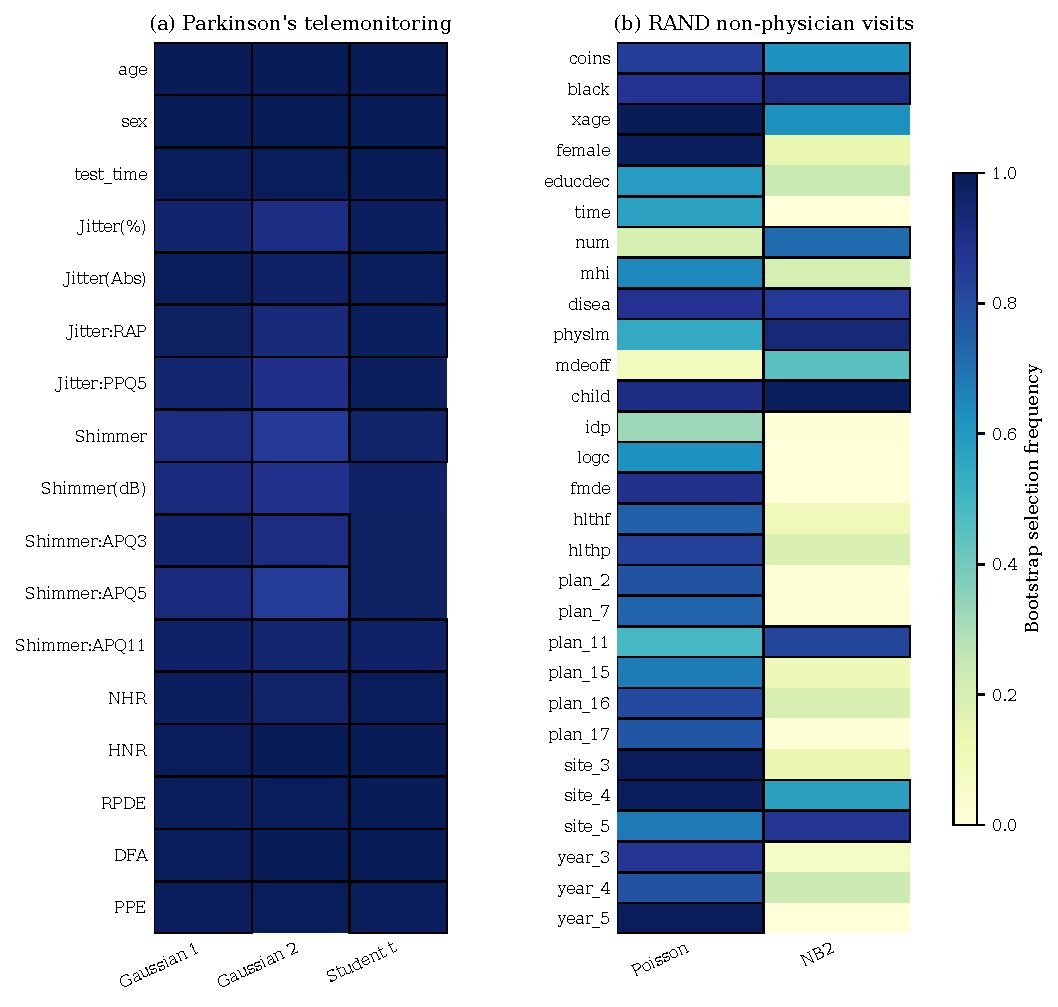
\includegraphics[width=\linewidth]{fig5.pdf}
\caption{Complete-pipeline bootstrap selection frequencies for slopes active in each full-data selected model. Black cell borders mark full-data inclusion. Participant clusters are resampled for Parkinson's telemonitoring; independent rows are resampled for RAND. The family tuple is fixed, while screening, tuning, support selection, and refitting are repeated.}
\label{fig:bootstrap-support}
\end{figure}

\section{Discussion and conclusions}
\label{sec:discussion}

This paper develops a frequentist framework for finite regression mixtures whose components need not share a response family. The framework preserves an interpretable regression within each latent component while allowing heterogeneity in dispersion, tail weight, skewness, and zero inflation. Its computational contribution is an integrated candidate-search pipeline with response-guided initialization, component-specific sparse supports, active-set likelihood refits, family-correct prediction, and analytical observed information. Its theoretical contribution is deliberately conditional: likelihood results are proved for a fixed, regular, identifiable family tuple, and the nonregular selection layers are named rather than absorbed into a generic regularity clause.

The simulations support three conclusions. First, family recovery can improve sharply with sample size, although exact labels are an incomplete target when a broader family approaches a simpler one at a boundary. Reporting strict and declared-equivalence recovery together makes that ambiguity visible. Second, componentwise lasso regularization substantially reduces false selections, but sparsity and predictive score need not improve together. Third, the analytical Louis calculation delivers calibrated fixed-model intervals in the representative real, positive, and count mixtures studied here. Direct derivative validation across all fourteen families and agreement with numerical Hessians in the Gaussian--Student-$t$ and Poisson--ZIP experiments help distinguish implementation accuracy from finite-sample mixture behavior.

The applications provide different strengths of evidence. In RAND, Poisson--NB2 leads the full-data BIC leaderboard, beats the best identical mixture in four of five splits, retains predictors in both components, and yields a bootstrap-stable overdispersed minority. Predictive differences from the best identical count mixture are small, which is compatible with BIC selecting a more parsimonious distributional representation. In Parkinson's telemonitoring, Gaussian--Gaussian--Student-$t$ leads the full-data BIC ranking, but the family-class advantage varies across participant splits and does not extend to RMSE or average log score. The exact support differences are also unstable, and the Student-$t$ degrees of freedom lies at the lower safeguard. This example is evidence that the enlarged model class can reveal a heavy-tailed latent structure; it is not decisive validation of one family tuple or a basis for coefficient-level clinical interpretation.

Several limitations identify concrete next steps. Constant mixing proportions do not let covariates explain component membership; a mixture-of-experts extension would add that mechanism. The applications use one common absolute penalty across components even though their effective sample sizes differ. Component-specific or effective-sample-size-scaled penalties may preserve meaningful slopes in smaller components and should be studied with theory appropriate to their tuning. We do not enlarge the reported tuning grid after seeing the data: the RAND bootstrap concentration at its largest prespecified value is disclosed as a sensitivity issue rather than used to justify a post hoc grid change.

The Parkinson likelihood treats repeated recordings as conditionally independent. Participant-grouped splitting and cluster bootstrap protect validation and uncertainty summaries from resampling recordings across subjects, but they do not replace a longitudinal likelihood with random effects or within-participant dependence. The RAND analysis screens a moderately large candidate set and therefore conditions its final bootstrap on the validated family pair. Neither bootstrap repeats family and component-number selection, so it is selection-aware for variables and tuning but not fully unconditional.

Finally, exhaustive tuple search grows combinatorially and every EM-type algorithm can settle at a local mode. Beam search and response-cluster starts reduce cost but do not certify a global optimum. Stronger global optimization, singular model-selection criteria, family-selection bootstrap, and selective or debiased inference remain open problems. Within these limits, component-specific response families offer a useful middle ground between a homogeneous-family mixture and a fully nonparametric conditional density. The practical recommendation is to report structure, prediction, support stability, and fixed-model uncertainty as distinct inferential objects. Their disagreement is often the most informative part of the analysis.

\section*{Data and code availability}

The implementation, simulation and application scripts, high-performance-computing job specifications, compact frozen result record, and figure-generation code are available at \url{https://github.com/samyajoypal/mixglm}. The tracked publication snapshot is under \texttt{experiments/paper\_figures/csda\_data}; \texttt{freeze\_csda\_results.py} rebuilds it from completed raw runs, and \texttt{make\_csda\_figures.py} rebuilds the sequential figures without refitting. The Supplementary Material gives exact paths and commands. The Parkinson's telemonitoring data are publicly available from the University of California, Irvine (UCI) Machine Learning Repository \citep{uci2009parkinsons}; the RAND variables are distributed with the data sources described by \citet{deb2002health} and \citet{cameron2005microeconometrics}.

\section*{Declaration of competing interest}

The authors declare that they have no known competing financial interests or personal relationships that could have appeared to influence the work reported in this paper.

\appendix

\section{Analytical Louis blocks and weighted M-step equations}
\label{app:analytic}

This appendix makes the analytical interface in Theorem~\ref{thm:louis} explicit. It first lists the family-level scores and Hessians in the transformed nuisance coordinates used by the optimizer, then gives the weighted regression and nuisance equations used in the M-step. Supplementary Section~S2 derives each block from its log density and reports independent finite-difference checks.

\subsection{Notation}
\label{app:notation}

For one response in one component, write
\[
 \ell=\log f(y;\mu,\gamma),\qquad
 a_\mu=\frac{\partial\ell}{\partial\mu},\qquad
 b_{\mu\mu}=\frac{\partial^2\ell}{\partial\mu^2},
\]
\[
 a_\gamma=\frac{\partial\ell}{\partial\gamma},\qquad
 B_{\gamma\gamma}=\frac{\partial^2\ell}{\partial\gamma\,\partial\gamma^\T},
 \qquad b_{\mu\gamma}=\frac{\partial^2\ell}{\partial\mu\,\partial\gamma}.
\]
Unlisted cross-derivatives are zero. Positive nuisance parameters are differentiated after a log transformation; inflation probabilities are differentiated after a logit transformation. The functions $\psi$ and $\psi_1$ are the digamma and trigamma functions, and $\varphi$ and $\Phi$ are the standard Gaussian density and distribution function.

\subsection{Family-specific derivative blocks}
\label{app:family-blocks}

The following fourteen blocks, combined with Proposition~\ref{prop:chain}, supply the complete-data component contributions needed in \eqref{eq:louis}. The parameterization in each block is the one used in estimation and simulation.

\paragraph{Gaussian.}
For $N(\mu,\sigma^2)$, let $v=\sigma^2=\exp(s)$ and $r=y-\mu$. Then
\[
 a_\mu=r/v,\qquad b_{\mu\mu}=-1/v,
\]
\[
 a_s=-\frac12+\frac{r^2}{2v},\qquad
 B_{ss}=-\frac{r^2}{2v},\qquad b_{\mu s}=-r/v.
\]

\paragraph{Student-$t$.}
Let $\sigma=\exp(a)$, $\nu=2+\exp(b)$, $w=\exp(b)$, $r=y-\mu$, $D=\nu\sigma^2+r^2$, $u=r^2/\sigma^2$, and $q=1+u/\nu$. The location and log-scale entries are
\[
 a_\mu=\frac{(\nu+1)r}{D},\qquad
 b_{\mu\mu}=\frac{(\nu+1)(r^2-\nu\sigma^2)}{D^2},
\]
\[
 a_a=-1+\frac{(\nu+1)r^2}{D},\qquad
 B_{aa}=-\frac{2(\nu+1)r^2\nu\sigma^2}{D^2},\qquad
 b_{\mu a}=-\frac{2(\nu+1)r\nu\sigma^2}{D^2}.
\]
Define
\[
 L_\nu=\frac12\psi\!\left(\frac{\nu+1}{2}\right)
 -\frac12\psi\!\left(\frac\nu2\right)-\frac{1}{2\nu}
 -\frac12\log q+\frac{(\nu+1)u}{2\nu(\nu+u)}
\]
and
\[
 \begin{split}
 L_{\nu\nu}={}&\frac14\psi_1\!\left(\frac{\nu+1}{2}\right)
 -\frac14\psi_1\!\left(\frac\nu2\right)+\frac{1}{2\nu^2}
 +\frac{u}{2\nu(\nu+u)}\\
 &+\frac{\tfrac12u\nu(\nu+u)-\tfrac12u(\nu+1)(2\nu+u)}
 {\{\nu(\nu+u)\}^2}.
 \end{split}
\]
The transformed degrees-of-freedom entries are
\[
 a_b=wL_\nu,\qquad B_{bb}=wL_\nu+w^2L_{\nu\nu},
\]
\[
 b_{\mu b}=\frac{w r(r^2-\sigma^2)}{D^2},\qquad
 B_{ab}=\frac{w r^2(r^2-\sigma^2)}{D^2}.
\]

\paragraph{Poisson.}
For $Y\sim\operatorname{Poisson}(\mu)$,
\[
 a_\mu=y/\mu-1,\qquad b_{\mu\mu}=-y/\mu^2.
\]

\paragraph{Negative binomial with quadratic variance.}
For $\Var(Y)=\mu+\alpha\mu^2$, let $\rho=\log\alpha$, $r=\alpha^{-1}=\exp(-\rho)$, and $A=r+\mu$. Then
\[
 a_\mu=\frac{y}{\mu}-\frac{r+y}{A},\qquad
 b_{\mu\mu}=-\frac{y}{\mu^2}+\frac{r+y}{A^2}.
\]
With
\[
 L_r=\psi(y+r)-\psi(r)+\log r+1-\log A-\frac{r+y}{A},
\]
\[
 L_{rr}=\psi_1(y+r)-\psi_1(r)+1/r-1/A-(\mu-y)/A^2,
\]
the transformed dispersion entries are
\[
 a_\rho=-rL_r,\qquad B_{\rho\rho}=rL_r+r^2L_{rr},\qquad
 b_{\mu\rho}=r(\mu-y)/A^2.
\]

\paragraph{Gamma.}
For the mean-shape Gamma model with $\kappa=\exp(a)$,
\[
 \ell=(\kappa-1)\log y-\kappa y/\mu-\log\Gamma(\kappa)
 -\kappa\log\mu+\kappa\log\kappa.
\]
Let
\[
 L_\kappa=\log y-y/\mu-\psi(\kappa)-\log\mu+\log\kappa+1,
 \qquad L_{\kappa\kappa}=-\psi_1(\kappa)+1/\kappa.
\]
Then
\[
 a_\mu=\kappa(y-\mu)/\mu^2,\qquad
 b_{\mu\mu}=\kappa(\mu-2y)/\mu^3,
\]
\[
 a_a=\kappa L_\kappa,\qquad
 B_{aa}=\kappa L_\kappa+\kappa^2L_{\kappa\kappa},\qquad
 b_{\mu a}=a_\mu.
\]

\paragraph{Exponential.}
For the exponential distribution parameterized by its mean,
\[
 a_\mu=(y-\mu)/\mu^2,\qquad b_{\mu\mu}=(\mu-2y)/\mu^3.
\]

\paragraph{Lognormal.}
Here $\mu$ denotes log-location. Let $\sigma=\exp(a)$ and $r=\log y-\mu$. Then
\[
 a_\mu=r/\sigma^2,\qquad b_{\mu\mu}=-1/\sigma^2,
\]
\[
 a_a=-1+r^2/\sigma^2,\qquad
 B_{aa}=-2r^2/\sigma^2,\qquad
 b_{\mu a}=-2r/\sigma^2.
\]

\paragraph{Inverse Gaussian.}
For mean $\mu$ and shape $\lambda=\exp(a)$, let $A=(y-\mu)^2/(2\mu^2y)$. Then
\[
 a_\mu=\lambda(y-\mu)/\mu^3,\qquad
 b_{\mu\mu}=\lambda(2\mu-3y)/\mu^4,
\]
\[
 a_a=1/2-\lambda A,\qquad B_{aa}=-\lambda A,\qquad b_{\mu a}=a_\mu.
\]

\paragraph{Bernoulli.}
For success probability $\mu$,
\[
 a_\mu=\frac{y}{\mu}-\frac{1-y}{1-\mu},\qquad
 b_{\mu\mu}=-\frac{y}{\mu^2}-\frac{1-y}{(1-\mu)^2}.
\]

\paragraph{Geometric.}
For the law on $\{0,1,\ldots\}$ parameterized by mean $\mu$,
\[
 a_\mu=y/\mu-(y+1)/(1+\mu),\qquad
 b_{\mu\mu}=-y/\mu^2+(y+1)/(1+\mu)^2.
\]

\paragraph{Beta.}
For the mean-precision parameterization, let $\phi=\exp(a)$, $A=\mu\phi$, and $B=(1-\mu)\phi$. Define
\[
 G=-\psi(A)+\psi(B)+\log y-\log(1-y),
\]
\[
 L_\phi=\psi(\phi)-\mu\psi(A)-(1-\mu)\psi(B)
 +\mu\log y+(1-\mu)\log(1-y),
\]
\[
 L_{\phi\phi}=\psi_1(\phi)-\mu^2\psi_1(A)-(1-\mu)^2\psi_1(B).
\]
Then
\[
 a_\mu=\phi G,\qquad
 b_{\mu\mu}=-\phi^2\{\psi_1(A)+\psi_1(B)\},
\]
\[
 a_a=\phi L_\phi,\qquad B_{aa}=\phi L_\phi+\phi^2L_{\phi\phi},
\]
\[
 b_{\mu a}=\phi G+\phi^2\{-\mu\psi_1(A)+(1-\mu)\psi_1(B)\}.
\]

\paragraph{Zero-inflated Poisson.}
Let $\zeta=\operatorname{logit}(\vartheta)$ and $\dot\vartheta=\vartheta(1-\vartheta)$. For $y>0$,
\[
 a_\mu=y/\mu-1,\qquad b_{\mu\mu}=-y/\mu^2,\qquad
 a_\zeta=-\vartheta,\qquad B_{\zeta\zeta}=-\dot\vartheta.
\]
For $y=0$, set
\[
 e=\exp(-\mu),\quad A=\vartheta+(1-\vartheta)e,\quad
 B=(1-\vartheta)e,
\]
\[
 C=\dot\vartheta(1-e),\qquad
 C_\zeta=\dot\vartheta(1-2\vartheta)(1-e).
\]
Then
\[
 a_\mu=-B/A,\qquad b_{\mu\mu}=B\vartheta/A^2,
\]
\[
 a_\zeta=C/A,\qquad
 B_{\zeta\zeta}=(C_\zeta A-C^2)/A^2,
 \qquad b_{\mu\zeta}=(\dot\vartheta eA+CB)/A^2.
\]

\paragraph{Zero-inflated negative binomial.}
For $y>0$, use the NB2 block and add
\[
 a_\zeta=-\vartheta,\qquad B_{\zeta\zeta}=-\vartheta(1-\vartheta).
\]
For $y=0$, let $r=\alpha^{-1}$, $p_0=\{r/(r+\mu)\}^r$, and
\[
 A=\vartheta+(1-\vartheta)p_0,\quad
 C=\dot\vartheta(1-p_0),\quad
 C_\zeta=\dot\vartheta(1-2\vartheta)(1-p_0).
\]
Let $g_j$ and $H_{j\ell}$ be the NB2 score and Hessian entries of $\log p_0$ for $j,\ell\in\{\mu,\rho\}$. Define
\[
 A_j=(1-\vartheta)p_0g_j,\qquad
 A_{j\ell}=(1-\vartheta)p_0(H_{j\ell}+g_jg_\ell),
 \qquad A_{j\zeta}=-\dot\vartheta p_0g_j.
\]
The zero-count block is
\[
 a_j=A_j/A,\qquad B_{j\ell}=(A_{j\ell}A-A_jA_\ell)/A^2,
\]
\[
 a_\zeta=C/A,\qquad B_{\zeta\zeta}=(C_\zeta A-C^2)/A^2,
 \qquad B_{j\zeta}=(A_{j\zeta}A-A_jC)/A^2.
\]
For completeness, with $D=r+\mu$ and
\[
 L_{r0}=\log r+1-\log D-r/D,
\]
the base zero-count entries are
\[
 g_\mu=-r/D,\quad H_{\mu\mu}=r/D^2,\quad
 g_\rho=-rL_{r0},\quad H_{\mu\rho}=r\mu/D^2,
\]
\[
 H_{\rho\rho}=rL_{r0}+r^2\{1/r-1/D-\mu/D^2\}.
\]

\paragraph{Skew normal.}
For the Azzalini skew-normal model, let $\omega=\exp(a)$, let $\alpha$ be shape, set $z=(y-\mu)/\omega$ and $t=\alpha z$, and define the inverse Mills ratio
\[
 M(t)=\varphi(t)/\Phi(t),\qquad M'(t)=-M(t)\{t+M(t)\}.
\]
With
\[
 \ell_z=-z+\alpha M(t),\qquad
 \ell_{zz}=-1+\alpha^2M'(t),\qquad
 \ell_{z\alpha}=M(t)+\alpha zM'(t),
\]
the block is
\[
 a_\mu=-\ell_z/\omega,\qquad b_{\mu\mu}=\ell_{zz}/\omega^2,
\]
\[
 a_a=-1-z\ell_z,\qquad a_\alpha=zM(t),
\]
\[
 B_{aa}=z\ell_z+z^2\ell_{zz},\qquad
 B_{\alpha\alpha}=z^2M'(t),\qquad
 B_{a\alpha}=-z\ell_{z\alpha},
\]
\[
 b_{\mu a}=(\ell_z+z\ell_{zz})/\omega,\qquad
 b_{\mu\alpha}=-\ell_{z\alpha}/\omega.
\]

\subsection{Weighted M-step equations}
\label{app:mstep}

At a GEM iteration, component $k$ receives weights $w_i=\tau_{ik}$. Its regression and nuisance update solves
\begin{equation}
 (\beta_k^+,\gamma_k^+)\in\argmax_{\beta,\gamma}
 \left\{\sum_{i=1}^n w_i\ell_{d_k}\{y_i;h_{d_k}(x_i^\T\beta),\gamma\}
 -\lambda_k\rho_{\alpha_k}(\beta_{-0})\right\}.
 \label{eq:weighted-mstep}
\end{equation}
The intercept is unpenalized. Define
\[
 U_{\eta i}=a_{\mu i}\dot h_i,\qquad
 J_{\eta i}=-\{b_{\mu\mu,i}\dot h_i^2+a_{\mu i}\ddot h_i\}.
\]
The unpenalized regression score and negative Hessian are
\[
 U_\beta=\sum_iw_ix_iU_{\eta i},
 \qquad J_{\beta\beta}=\sum_iw_ix_ix_i^\T J_{\eta i}.
\]
Whenever $J_{\eta i}>0$, a Newton/IRLS step has working response and weight
\[
 z_i=x_i^\T\beta+U_{\eta i}/J_{\eta i},
 \qquad \widetilde w_i=w_iJ_{\eta i}.
\]
For an unpenalized active coordinate set $\A$,
\[
 \beta_\A^+=\argmin_b\frac12\sum_i\widetilde w_i(z_i-x_{i,\A}^\T b)^2.
\]
For ridge, this is the corresponding penalized normal equation with a zero penalty on the intercept. For lasso, coordinate descent on the quadratic surrogate gives, for $j>0$,
\[
 \beta_j^+=
 \frac{S\!\left\{\sum_i\widetilde w_i x_{ij}
 (z_i-\sum_{\ell\neq j}x_{i\ell}\beta_\ell),\lambda_k\right\}}
 {\sum_i\widetilde w_i x_{ij}^2},
 \qquad S(u,\lambda)=\operatorname{sign}(u)(|u|-\lambda)_+.
\]
For elastic net, the threshold is $\lambda_k\alpha_k$ and the denominator gains $\lambda_k(1-\alpha_k)$.

Several familiar updates follow directly. With an identity-link Gaussian component, weighted least squares updates $\beta_k$ and
\[
 (\sigma_k^2)^+=\frac{\sum_iw_i(y_i-x_i^\T\beta_k^+)^2}{\sum_iw_i}.
\]
With canonical Bernoulli or Poisson links, the displayed IRLS equations reduce to their usual responsibility-weighted forms. Lognormal regression is weighted least squares for $\log y$ and has
\[
 (\sigma_k^2)^+=\frac{\sum_iw_i(\log y_i-x_i^\T\beta_k^+)^2}{\sum_iw_i}.
\]
For nuisance parameters without a closed-form maximizer, the low-dimensional update solves
\[
 U_\gamma(\beta,\gamma)=\sum_iw_i a_{\gamma i}=0,
 \qquad
 H_{\gamma\gamma}(\beta,\gamma)=\sum_iw_iB_{\gamma\gamma,i},
\]
using safeguarded Newton or the limited-memory Broyden--Fletcher--Goldfarb--Shanno (BFGS) algorithm with the analytical cross-block $\sum_iw_i\dot h_i x_i b_{\mu\gamma,i}^\T$. This covers Student-$t$ scale and degrees of freedom, NB2 dispersion, Gamma shape, inverse-Gaussian shape, beta precision, zero-inflation probability, and skew-normal scale and shape. A proposed block is accepted only if it increases \eqref{eq:qfun}, which is the condition used in Theorem~\ref{thm:gem}.

\bibliographystyle{cas-model2-names}
\bibliography{references}

\end{document}
